\chapter{Related Work}
\label{rw:intro}

In this chapter relevant work related to the thesis topic will be briefly presented. In section
\ref{rw:logicProgramming}...


\section{Logic Programming}
\label{rw:logicProgramming}

\cite{DBLP:books/sp/Lloyd87}
\cite{DBLP:journals/ml/LavracD96}
In this section, basic logic programming and deductive database terminology such as \emph{literal}, \emph{clause},
\emph{program clause}, \emph{datalog clause} and \emph{hypothesis} will be presented. Firstly, it is important to
mention that variables are represented as uppercase letters followed by a string of lowercase letters and/or digits.
Function and predicate symbols are lowercase letters also followed by a string of lowercase and/or digits.

An \emph{atomic formula} $L$ is a predicate symbol followed by a bracketed n-tuple of \emph{terms}. A \emph{term} can be
a variable or a function symbol followed by a bracketed n-tuple of terms. A constant is a function symbol of arity 0. So
for example, if $f$, $g$, and $h$ are function symbols and $X$ a variable, then $g(X)$ is term, $f(g(X),h)$ is also a
term and $h$ is a \emph{constant}.

A \emph{literal} is an \emph{atomic formula} which can be negated or not. So both $L$ and its negation $\overline{L}$
are literals for any \emph{atomic formula} $L$. A clause $c$ is a disjunction of literals, for example:
\begin{center}
  $c=(L_1 \vee L_2 \vee \ldots \overline{L_{i}} \vee \overline{L_{i+1}} \vee \ldots) \equiv
 L_1 \vee L_2 \vee \ldots \leftarrow L_i \wedge L_{i+1} \wedge \ldots$
\end{center}

Such disjunction of literals can also be written in following way:
\begin{center}
 $\{L_1,L_2,\ldots,\overline{L_i},\overline{L_{i+1}},\ldots\}$ \\
$ L_1,L_2,\ldots \leftarrow L_i,L_{i+1},\ldots$
\end{center}

A \emph{program clause} is a clause which contains exactly one positive literal. That is, it has the form:
\begin{center}
 $\underbrace{T}_{head} \leftarrow \underbrace{L_1,L_2,\ldots}_{body}$
\end{center}

A \emph{datalog clause} is a program clause with no function symbols with arity greater different from zero. That means
that only variables and constants can be used as predicate arguments. A datalog clause is considered $safe$ if all the
variables present in the head literal $T$ are also present in the body. Moreover, it may also allow negated literals in
the body, as long as every variable existent in a negated body literal are also be present in a non-negated body
literal.

\section{Inductive Logic Programming}

\cite{DBLP:journals/ml/LavracD96}
Inductive Logic Programming (ILP) is a machine learning technique that combines inductive machine learning with the
logic programming representation. Given a known background knowledge and a set of training examples represented as a
logical database of facts (literals without any variables), an ILP system will learn a hypothesis in the form of a
logic program.

The clauses in the hypothesis aim at recognizing a concept $\mathcal{C}$, which is defined as a subset of objects
$\mathcal{C} \subseteq \mathcal{U}$. For example, $\mathcal{U}$ may be the set of all students in a University and
$\mathcal{C}$ all the students studying Informatics.
Concepts and objects are described in a description language $\mathcal{L}$, typically a subset of first-order logic, but
various languages have also been used in ILP, including propositional logic and first order predicate calculus.

The training data for learning a concept $\mathcal{C}$ is a set of examples $\mathcal{E}$, where each examples is a
grounded fact
labeled as positive ($\oplus$) if the object is an instance of $\mathcal{C}$, or negative ($\ominus$) otherwise. We
denote the set
of positive examples as $\mathcal{E}^{+}$ and the set of negative examples as $\mathcal{E}^{-}$.

The background knowledge $\mathcal{B}$ is a prior knowledge which contributes in learning the hypothesis. It indirectly
restricts the hypothesis search space, as  the learned hypothesis $\mathcal{H}$ should be consistent with the background
knowledge as well as the training examples.

A hypothesis $\mathcal{H}$ is said to cover an example $e$ given a background knowledge
$\mathcal{B}$ ($covers(\mathcal{B} \cup \mathcal{H},e)$) if the example satisfies the hypothesis and background
knowledge. In logic programming where the $\mathcal{H}$ is a set of program clauses and an example is a ground fact, it
means that $e$ is entailed by $\mathcal{B} \cup \mathcal{H}$.

\begin{center}
 $covers(\mathcal{B} \cup \mathcal{H},e)=true \quad$ if $\quad \mathcal{B} \cup \mathcal{H} \models e$
\end{center}

We can also define a covering function for a set of examples which returns a a subset with the examples entailed by
$\mathcal{B} \cup \mathcal{H}$:

\begin{center}
 $covers(\mathcal{B} \cup \mathcal{H},\mathcal{E})=\{e \in \mathcal{E} | \mathcal{B} \cup \mathcal{H} \models e\}$
\end{center}

Therewith, we can define two important concepts in inductive learning:

\begin{itemize}
 \item Completeness: A hypothesis $\mathcal{H}$ is complete with respect to background knowledge $\mathcal{B}$ and
examples $\mathcal{E}$ if all the positive examples are covered, or in other words:
$covers(\mathcal{B},\mathcal{H},\mathcal{E}^{+})=\mathcal{E}^{+}$
 \item Consistency: A hypothesis $\mathcal{H}$ is consistent with respect to background knowledge $\mathcal{B}$ and
examples $\mathcal{E}$ if no negative examples are covered, or in other words:
$covers(\mathcal{B},\mathcal{H},\mathcal{E}^{-})=\emptyset$
\end{itemize}

The objective of learning a concept requires a hypothesis that is complete and consistent with respect to the given
concept training examples and background knowledge. The example shown in table \ref{tb:ilpExample} (presented in
\cite{DBLP:journals/ml/LavracD96}) illustrates a simple problem of learning a hypothesis for the target relation
$daughter(X,Y)$.

\begin{table}[h!]
\label{tb:ilpExample}
\caption{A simple ILP problem: learning the \emph{daughter} relation.}
  \begin{center}
      \begin{tabular}{ r | l }
      \toprule
      \textbf{Training Examples} & \textbf{Background Knowledge}\\
      \midrule
      daughter(mary,ann) $\oplus$	& parent(ann,mary).	\\
      daughter(eve,tom) $\oplus$	& parent(ann,tom).	\\
      daughter(tom,ann) $\ominus$ 	& parent(tom,eve).	\\
      daughter(eve,ann) $\ominus$	& parent(tom,ian).	\\
					& female(ann).		\\
					& female(mary).		\\
					& female(eve).		\\
      \bottomrule
      \end{tabular}
  \end{center}
\end{table}

If we consider, for example, the language of safe datalog clauses, it is possible to formulate the following complete
and consistent hypothesis:

\begin{center}
  $\mathcal{H} = daughter(X,Y)$ :- $female(X),parent(Y,X)$ 
\end{center}

\subsection{Searching the Hypothesis Space}

In ILP, the hypothesis space is determined by the language of the programs $\mathcal{L}$ consisting of the possible
program clauses allowed by the language. Also, the vocabulary of predicate symbols is determined by the predicates from
the background knowledge $\mathcal{B}$.

It is useful to structure the search space with partial ordering into a set of clauses based on $\theta$-subsumption in
order to systematically search the program clauses space. A clause $c$ $\theta$-subsumes $c'$ if there's a
substitution $\theta$ such that clause $c\theta \subseteq c'$. This also introduces a notion of generality, where
clause $c$ is at least as generaly as $c'$, or in other words, $c'$ is a specialization of $c$.

For example, if we have the following $c$ and $c'$:
\begin{align*}
  c &= daughter(X,Y) \text{ :- } parent(Y,X) \\
  c'&= daughter(X,Y )\text{ :- } female(X),parent(Y,X)
\end{align*}

we know taht for that $c'$ is a specialization of $c$ because for $\theta=\emptyset$, $c \subset c'$ since:
\begin{center}
$\{daughter(X,Y),\neg parent(Y,X)\} \subset \{daughter(X,Y),\neg female(X),\neg parent(Y,X)\}$ 
\end{center}

To better illustrate it, if we have:
\begin{align*}
  c &= livesIn(X,Y) \text{ :- } marriedTo(X,Z),livesIn(Z,Y)\\
  c'&=livesIn(X,germany) \text{ :- } marriedTo(X,Z),livesIn(Z,germany)
\end{align*}

we know that $c'$ is a specialization of $c$ because with the substitution $\theta=\{Y/germany\}$, $c\theta=c'$.

This notion gives us an important property that can be used for pruning parts of the search space:

\begin{itemize}
 \item When generalizing from $c$ to $c'$, all the examples covered by $c$ are also covered by $c'$. So if $c$ is
inconsistent, then all its generalizations are inconsistent as well.
  \item When specializing from $c$ to $c'$, an example not covered by $c$ will neither be covered by $c'$. So if $c'$
does not cover any positive examples, neither do any its specializations.
\end{itemize}

These properties are the basis for two main search approaches:

\begin{itemize}
 \item Bottom-up: starts with less general clauses and searches least general generalizations
 \item Top-down: starts with more general clauses and searches for most general consistent specializations
\end{itemize}

As in this thesis we work only with the top-down approach, we will discuss it in more details in the next subsection.
Further information about bottow-up approach can be found in \cite{DBLP:journals/ml/LavracD96}.

\subsection{Top-Down ILP}

The search space of program clauses can be viewed as a lattice, structured by $\theta$-subsumption generality
ordering. Such lattice is called a \emph{refinement graph}, which can be used to direct the search from most general to
specific hypothesis. The figure \ref{fig:refinementGraph} illustrates a part of the refinement graph for the
family relation example shown in table \ref{tb:ilpExample}.

\begin{figure}[h!]
\label{fig:refinementGraph}
\begin{center}
  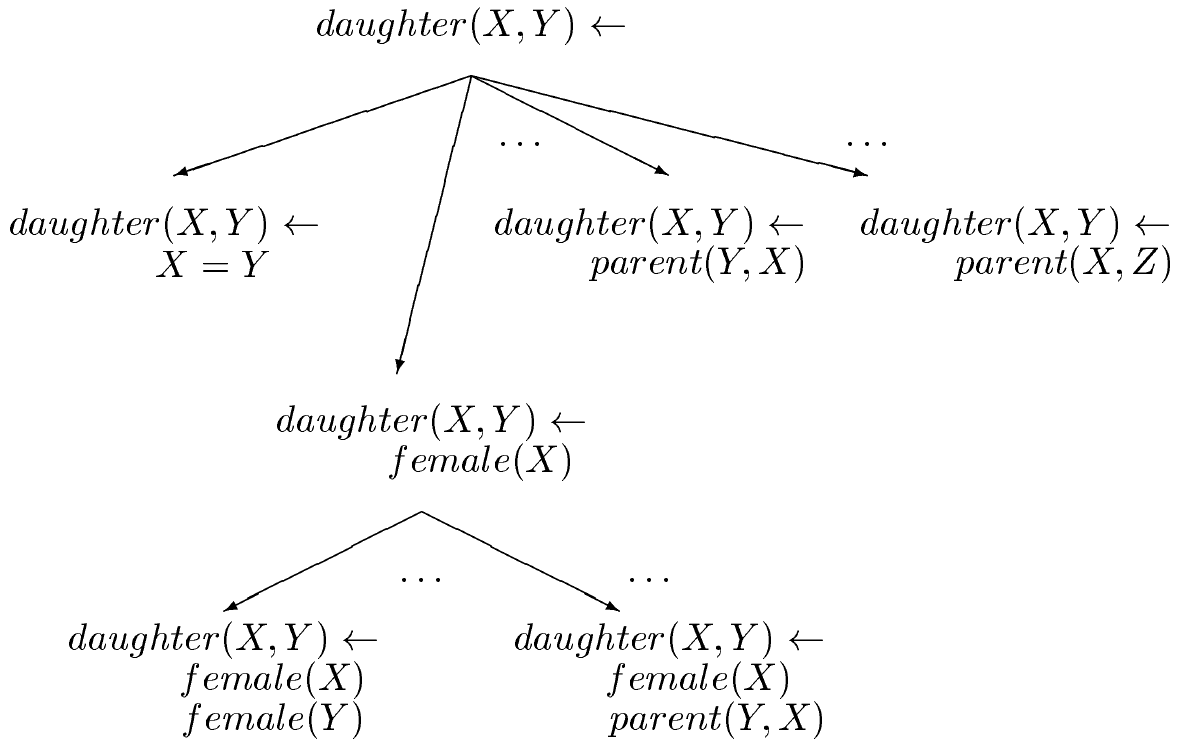
\includegraphics[width=0.7\linewidth]{./Figures/refinementGraph.png}
\end{center}
\caption{Part of the refinement graph for the family relations problem}
\end{figure}

In such graph, nodes are program clauses and arcs are refinement operations, which can be of two kinds:

\begin{itemize}
 \item Apply a substitution on the clause
 \item Add a literal to the body of the clause
\end{itemize}

The top-down algorithm consists basically of a specialization loop that refines a clause ensuring consistency
embedded inside a covering loop that adds clauses to the hypothesis ensuring completeness. Each loop has a stopping
criterion, the covering loop iterates until it satisfies a sufficiency criterion and the specialization loop iterates
until it satisfies a necessity criterion. The algorithm \ref{alg:topDownILP} shows in more details how the generic
top-down ILP works.

\begin{algorithm}[!h]
  \caption{Generic top-down specialization ILP algorithm}
  \label{alg:topDownILP}
  \SetKwFunction{executeQuery}
  \KwIn{\textbf{Input:} $\mathcal{E}$: Training examples, $\mathcal{B}$: Background knowledge \\ }
  \KwResult{$\mathcal{H}$: Learned hypothesis}

  \tcp{Initialize the current training set and hypothesis}
  $\mathcal{E}_{cur} \leftarrow \mathcal{E}$ \;
  $\mathcal{H} \leftarrow \emptyset$ \;
  \Repeat(Covering Loop){Sufficiency Stopping Criterion is satisfied} {
    \tcp{Initialize clause with empty body}
    $c \leftarrow T$ :- $\emptyset$ \;
    \Repeat(Specialization Loop){Necessity Stopping Criterion is satisfied} {
      $c_{best} \leftarrow$ Best refinement of $c$;
      $c \leftarrow c_{best}$ \;
    } ()
    \tcp{Add clause to the hypothesis}
    $\mathcal{H} \leftarrow \mathcal{H} \cup \{c\}$ \;
    \tcp{Remove positive examples covered by the new hypothesis}
    $\mathcal{E}_{cur} \leftarrow \mathcal{E}_{cur} - covers(\mathcal{B} \cup \mathcal{H},\mathcal{E}_{cur}^{+})$ \;
  } ()
\end{algorithm}

In domains with perfect data, the stopping criteria require that all positive examples are covered (completeness) and no
negative examples are covered (consistency). However, in practice many datasets have imperfect data. Such imperfection
is usually of the following kinds, as described in \cite{DBLP:conf/aii/LavracD92}:

\begin{itemize}
  \item Noise: random errors in the training examples and background knowledge
  \item Insufficiently covered example space: too sparse training examples from which it is difficult to reliably
detect correlations
  \item Inexactness: inappropriate or insufficient description language which does not contain an exact description of
the target concept
  \item Missing values in the training example
\end{itemize}

In order to avoid the effects of imperfect data, ILP can use heuristics as stopping criteria which tolerate
some level of incompleteness and inconsistency. The simplest heuristic is the expected accuracy of a clause, which is
defined as the probability that an example
covered by the clause is labeled as positive:
\begin{equation}
A(c)=P(e \in \mathcal{E}^{+}|c)=\cfrac{n^{+}(c)}{n^{+}(c)+n^{-}(c)} 
\end{equation}
where $n^{+}(c)$ is the number of positive and $n^{-}(c)$ the number of negative examples covered by $c$. 

\subsection{ILP Complexity}

As discussed in \cite{DBLP:journals/ngc/GottlobLS99}, the complexity of ILP resides at the second level of polynomial
hierarchy and it is $\Sigma_2^P$-complete. Thus, there are two sources of complexity:
\begin{itemize}
 \item Choice problem: 
 \item Checking problem: checking if a choice was good or not
\end{itemize}


As ILP complexity grows exponentially with the number of literals, it is common to restrict the number of literals
allowed in a clause in order to reduce execution time.
[Sampling,MaxLiterals]


%\section{First Order Inductive Learning}
%\cite{DBLP:journals/ml/Quinlan9}
%\cite{DBLP:conf/ecml/QuinlanC93}

\section{Association Rule Mining}
\cite{Agrawal:1993:MAR:170036.170072}
\cite{Hipp00algorithmsfor}

Association Rule Mining is method for discovering interesting relations between variables in large databases. It is
intended to work on a database composed by a set of transactions $\mathcal{D}=\{t_1,t_2,\ldots,t_m\}$ and a set of items
$\mathcal{I}=\{i_1,i_2,\ldots,i_n\}$. Each transaction $\mathcal{T}$ consists of a set of items which is subset of $I$ ,
which is usually represented by a binary vector of size $n$ indicating the presence of absence of items in the
transaction.

The objective of association rule mining is to learn inference rules of the form $X \Rightarrow Y$, where $X,Y
\subseteq I$ and $X \cap Y = \emptyset$. Rules are selected according to various interestingness measures that will be
subsequently discussed.

\subsection{Measures}

In this subsection we will discuss measures used for selecting interesting rules in the mining process.

We say a transaction $\mathcal{T}$ supports an itemset $\mathcal{X} \subseteq \mathcal{I}$ if $\mathcal{X} \subseteq
\mathcal{T}$. The support measure $supp(X)$ is the defined as the ratio between the number of transactions supporting
$X$ and the total size of the database $\mathcal{D}$:

\begin{equation}
 supp(X)=\cfrac{|\{ \mathcal{T} \in \mathcal{D} | X \subseteq \mathcal{T} \}|}{|\mathcal{D}|}
\end{equation}

The support of a rule $X \Rightarrow Y$ is defined as:

\begin{equation}
 supp(X \Rightarrow Y)=supp(X \cup Y)
\end{equation}

The confidence of a rule $X \Rightarrow Y$, which can may be interpreted as the probability of the the head given the
body $P(Y|X)$, is defined as:

\begin{equation}
 conf(X \Rightarrow Y)=\cfrac{supp(X \cup Y)}{sup(X)}
\end{equation}

%Need to cite who invented lift
Confidence and support are the two measures used in classical association rule mining. Albeit, there are other relevant
measures such as \emph{lift}. It measures how different the observed rule support is in comparison to that expected if
$X$ and $Y$ were independent:

\begin{equation}
 lift(X \Rightarrow Y)=\cfrac{supp(X \Rightarrow Y)}{supp(X)supp(Y)}
\end{equation}

A lift value 1 would imply that $X$ and $Y$ are independent, therefore any rule involving both itemsets does not make
sense. A lift value greater than 1, provides information about the level of dependence between both variables. Higher
lift values makes a rule potentially more interesting.

\subsection{Anti-monotonicity of Support}

An important characteristic of the support measure is the anti-monotonicity. It means that for any itemset $X
\subseteq \mathcal{I}$ if we have another itemset $Y \subseteq \mathcal{I}$ such that $X \subseteq Y$, then the support
of $Y$ cannot be greater than the support of $X$. In other words, all subsets from a frequent itemset are also frequent,
and all supersets from an infrequent item are also infrequent.

When searching for frequent itemsets, this characteristic plays a key role in pruning the search space, which grows
exponentially with the number of items $n$. The set of possible itemsets is the power set over $\mathcal{I}$, which has
size $2^n-1$. As association rules are usually required to satisfy a specified minimum support, if we know that a given
itemset does not satisfy it, we can automatically prune all its supersets.

\subsection{Itemset Lattice}

The problem of searching frequent itemsets (FI), i.e., itemsets that satisfy the specified minimum support, can be
structured in a lattice. Firstly, an itemset is frequent if it has support greater or equal than an arbitrarily
specified minimum support.


There are two special kinds of itemsets:
\begin{itemize}
 \item Maximal frequent itemset (MFI): a frequent itemset is maximal if none of its immediate supersets are frequent.
 \item Closed frequent itemset (CFI): a frequent itemset is closed if all of its immediate supersets have lower
support.
\end{itemize}

Each of these kinds of itemsets has an special property. By knowing all the maximal itemsets of a database, we
also know all the frequent itemsets. Nevertheless, it is not possible to know the support of each of the frequent
itemsets. By knowing all the closed of a database, it is possible to know the all the frequent itemsets as well as their
supports.

In the example of database $\mathcal{D}$ shown in table \ref{tb:itemsetLattice} with resulting itemset lattice shown in
figure \ref{fig:itemsetLattice}, frequent itemsets are shown with thicker border. The minimum support threshold was set
to $\cfrac{2}{5}$, so the frequent itemsets are the ones with frequency greater than or equal to 2. For this example, we
would have as maximal itemset $\{ABCE\}$ and as closed itemsets $\{ABCE, BCE, BE\}$

\begin{table}[h!]
  \begin{center}
    \label{tb:itemsetLattice}
      \begin{tabular}{ c | l l l l }
      \toprule
      \textbf{TID} & \multicolumn{4}{c}{\textbf{Items}} \\
      \midrule
	1	& A & C & D & \\
	2 	& B & C & E & \\
	3	& A & B & C & E \\
	4 	& B & E &   & \\
	5	& A & B & C & E \\
      \bottomrule
      \end{tabular}
  \caption{Example of transaction database $\mathcal{D}$ \cite{Pasquier99efficientmining}}
  \end{center}
\end{table}

\begin{figure}[!h]
  \caption{Itemset Lattice example}
  \centering
  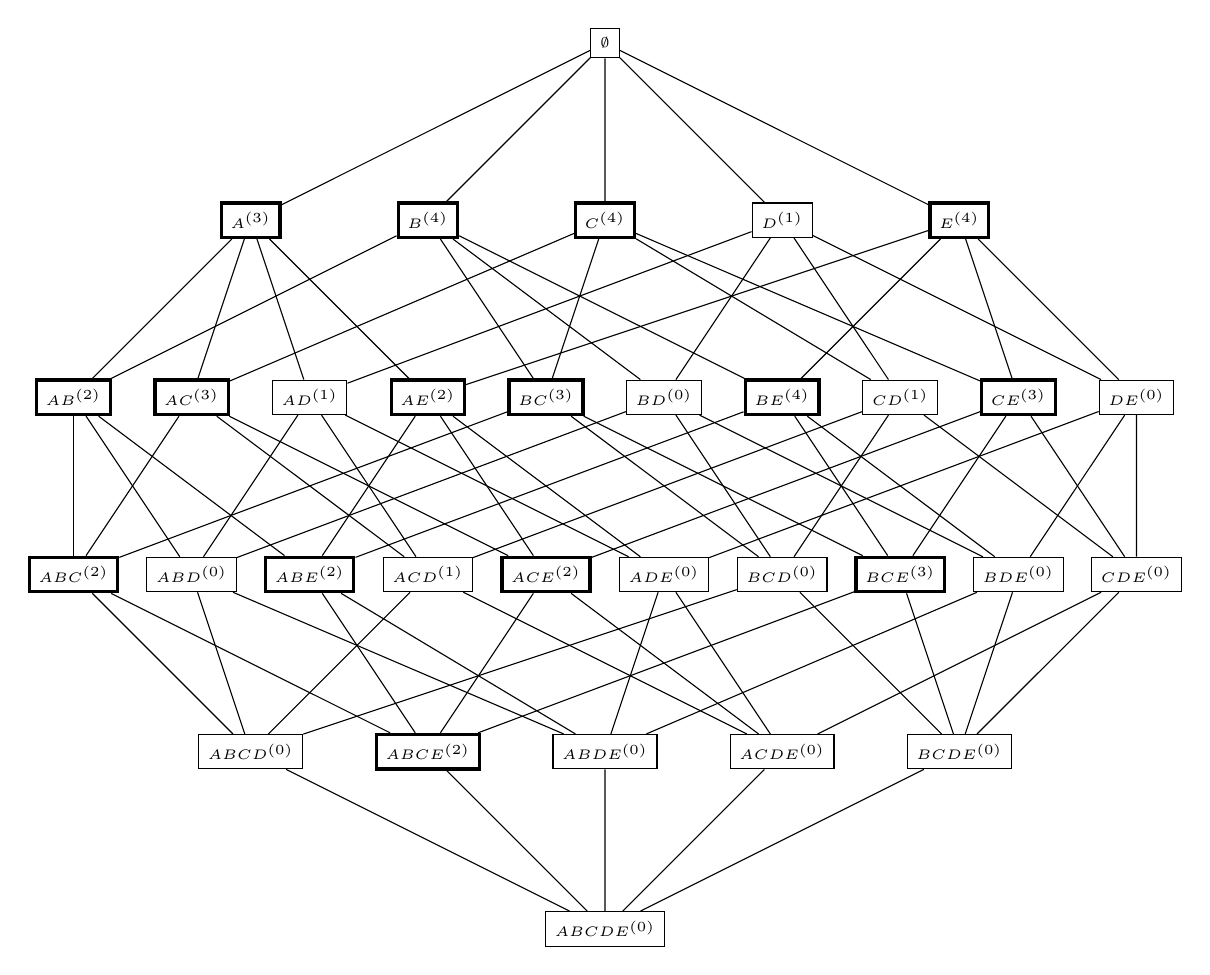
\begin{tikzpicture}[scale=0.75,auto=center,every node/.style={draw=black, font=\tiny}]
    \node (n0) at (11,15) {$\emptyset$};

    \node (A)[very thick] 	at (5,12)  {$A^{(3)}$};
    \node (B)[very thick] 	at (8,12)  {$B^{(4)}$};
    \node (C)[very thick]	at (11,12) {$C^{(4)}$};
    \node (D)			at (14,12) {$D^{(1)}$};
    \node (E)[very thick]	at (17,12) {$E^{(4)}$};

    \node (AB)[very thick] 	at (2,9)  {$AB^{(2)}$};
    \node (AC)[very thick] 	at (4,9)  {$AC^{(3)}$};
    \node (AD) 			at (6,9)  {$AD^{(1)}$};
    \node (AE)[very thick] 	at (8,9)  {$AE^{(2)}$};
    \node (BC)[very thick] 	at (10,9) {$BC^{(3)}$};
    \node (BD) 			at (12,9) {$BD^{(0)}$};
    \node (BE)[very thick] 	at (14,9) {$BE^{(4)}$};
    \node (CD) 			at (16,9) {$CD^{(1)}$};
    \node (CE)[very thick] 	at (18,9) {$CE^{(3)}$};
    \node (DE) 			at (20,9) {$DE^{(0)}$};

    \node (ABC)[very thick] 	at (2,6)  {$ABC^{(2)}$};
    \node (ABD) 		at (4,6)  {$ABD^{(0)}$};
    \node (ABE)[very thick] 	at (6,6)  {$ABE^{(2)}$};
    \node (ACD) 		at (8,6)  {$ACD^{(1)}$};
    \node (ACE)[very thick] 	at (10,6) {$ACE^{(2)}$};
    \node (ADE) 		at (12,6) {$ADE^{(0)}$};
    \node (BCD) 		at (14,6) {$BCD^{(0)}$};
    \node (BCE)[very thick] 	at (16,6) {$BCE^{(3)}$};
    \node (BDE) 		at (18,6) {$BDE^{(0)}$};
    \node (CDE) 		at (20,6) {$CDE^{(0)}$};

    \node (ABCD) 		at (5,3)  {$ABCD^{(0)}$};
    \node (ABCE)[very thick] 	at (8,3)  {$ABCE^{(2)}$};
    \node (ABDE) 		at (11,3) {$ABDE^{(0)}$};
    \node (ACDE) 		at (14,3) {$ACDE^{(0)}$};
    \node (BCDE) 		at (17,3) {$BCDE^{(0)}$};

    \node (ABCDE) at (11,0) {$ABCDE^{(0)}$};

    \foreach \from/\to in
      {n0/A,n0/B,n0/C,n0/D,n0/E,
       A/AB, A/AC, A/AD, A/AE, 
       B/AB, B/BC, B/BD, B/BE, 
       C/AC, C/BC, C/CD, C/CE,
       D/AD, D/BD, D/CD, D/DE,
       E/AE, E/BE, E/CE, E/DE,
       AB/ABC, AB/ABD, AB/ABE,
       AC/ABC, AC/ACD, AC/ACE,
       AD/ABD, AD/ACD, AD/ADE,
       AE/ABE, AE/ACE, AE/ADE,
       BC/ABC, BC/BCD, BC/BCE,
       BD/ABD, BD/BCD, BD/BDE,
       BE/ABE, BE/BCE, BE/BDE,
       CD/ACD, CD/BCD, CD/CDE,
       CE/ACE, CE/BCE, CE/CDE,
       DE/ADE, DE/BDE, DE/CDE,
       ABCD/ABC, ABCD/ABD, ABCD/ACD, ABCD/BCD,
       ABCE/ABC, ABCE/ABE, ABCE/ACE, ABCE/BCE,
       ABDE/ABD, ABDE/ABE, ABDE/ADE, ABDE/BDE,
       ACDE/ACD, ACDE/ACE, ACDE/ADE, ACDE/CDE,
       BCDE/BCD, BCDE/BCE, BCDE/BDE, BCDE/CDE,
       ABCDE/ABCD, ABCDE/ABCE, ABCDE/ABDE, ABCDE/ACDE, ABCDE/BCDE}  
    \draw (\from) -- (\to);
  \end{tikzpicture}
  \label{fig:itemsetLattice}
\end{figure}


[...]

\subsection{Apriori Algorithm}
The apriori algorithm is a method for searching frequent itemsets which explores the anti-monotonic property of the
support measure. It computeds the itemsets support iteratively, by ascending order of size. The
process takes $k$ iterations where $k$ is the size of the largest frequent itemset. In each iteration $i \leq k$, the
database is scanned once and all the support of all itemsets of size $i$ are computed.

In the first iteration, all itemsets of size 1 have their supports computed. On the $1 < i \leq k$ subsequent
iterations, a set of candidates $C_i$ is created by joining the frequent itemsets of size $i-1$ found in the previous
iteration. Two itemsets of size $i$ can only join if they share $i-1$ items, so their union can form an itemset of size
$i+1$. Only after finding the set of candidate itemsets $C_1$, the database is scanned in order to determine the
support of each of them. The algorithm \ref{alg:apriori} shows in more details how the apriori algorithm works.

\begin{algorithm}[h!]
  \caption{Apriori frequent itemset discovery}
  \label{alg:apriori}
  \SetKwFunction{aprioriGen}
  \KwIn{\textbf{Input:} $\mathcal{D}$: Database of transactions \\}
  \KwResult{$\mathcal{H}$: Learned hypothesis}

  $L_1 \leftarrow$ Frequent itemsets of size 1 \;
  $L \leftarrow L_1$ \;
  $k \leftarrow 1$ \;
  \While{$L_{k-1} \neq \emptyset$}{
      $C_k \leftarrow$ \FuncSty{aprioriGen(}$L_{k-1}$\FuncSty{)} \;
      \ForAll{$t \in \mathcal{D}$}{
	$C_t \leftarrow \{ c | c \in C_k \wedge c \subseteq t\}$ \;
	\ForAll{$c \in C_t$}{
	  $c.frequency \leftarrow c.frequency + 1$ \;
	}
      }
      $L_k \leftarrow \{ c | c \in C_k \wedge c.frequency \geq minSupport\}$ \;
      $L \leftarrow L \cup L_k$ \;
      $k \leftarrow k+1$ \;
  }
  \Return{$L$} \;
\end{algorithm}

For the previous example of database \ref{tb:aprioriLattice}, the itemset lattice generated by the apriori algorithm
is shown in figure \ref{fig:itemsetLattice}. 

\begin{figure}[h!]
  \caption{Itemset Lattice example}
  \centering
  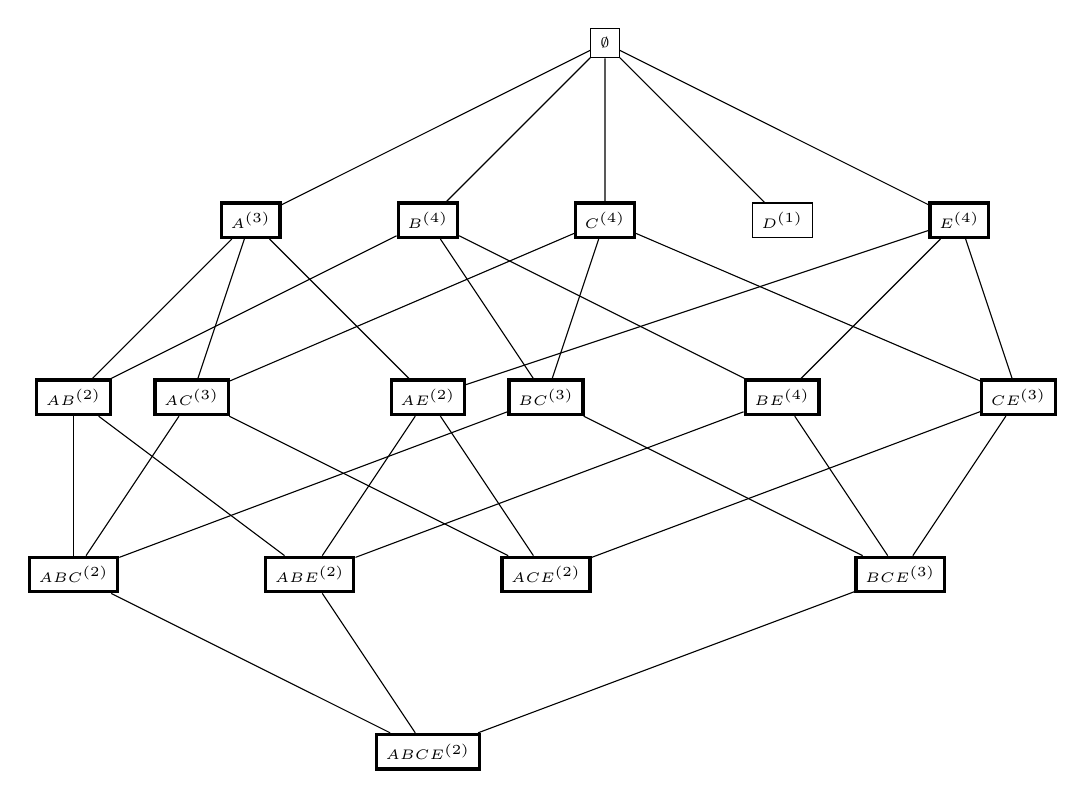
\begin{tikzpicture}[scale=0.75,auto=center,every node/.style={draw=black, font=\tiny}]
    \node (n0) at (11,15) {$\emptyset$};

    \node (A)[very thick] 	at (5,12)  {$A^{(3)}$};
    \node (B)[very thick] 	at (8,12)  {$B^{(4)}$};
    \node (C)[very thick]	at (11,12) {$C^{(4)}$};
    \node (D)			at (14,12) {$D^{(1)}$};
    \node (E)[very thick]	at (17,12) {$E^{(4)}$};

    \node (AB)[very thick] 	at (2,9)  {$AB^{(2)}$};
    \node (AC)[very thick] 	at (4,9)  {$AC^{(3)}$};
    \node (AE)[very thick] 	at (8,9)  {$AE^{(2)}$};
    \node (BC)[very thick] 	at (10,9) {$BC^{(3)}$};
    \node (BE)[very thick] 	at (14,9) {$BE^{(4)}$};
    \node (CE)[very thick] 	at (18,9) {$CE^{(3)}$};

    \node (ABC)[very thick] 	at (2,6)  {$ABC^{(2)}$};
    \node (ABE)[very thick] 	at (6,6)  {$ABE^{(2)}$};
    \node (ACE)[very thick] 	at (10,6) {$ACE^{(2)}$};
    \node (BCE)[very thick] 	at (16,6) {$BCE^{(3)}$};

    \node (ABCE)[very thick] 	at (8,3)  {$ABCE^{(2)}$};

    \foreach \from/\to in
      {n0/A,n0/B,n0/C,n0/D,n0/E,
       A/AB, A/AC, A/AE, 
       B/AB, B/BC, B/BE, 
       C/AC, C/BC, C/CE,
       E/AE, E/BE, E/CE,
       AB/ABC, AB/ABE,
       AC/ABC, AC/ACE,
       AE/ABE, AE/ACE,
       BC/ABC, BC/BCE,
       BE/ABE, BE/BCE,
       CE/ACE, CE/BCE,
       ABCE/ABC, ABCE/ABE, ABCE/BCE}  
    \draw (\from) -- (\to);
  \end{tikzpicture}
  \label{fig:aprioriLattice}
\end{figure}

\section{Mining Optimized Rules for Numeric Attributes}

In \cite{Brin99miningoptimized}, a technique for efficient learning association rules with interesting ranges for
numerical attributes is presented. It focuses on finding numerical intervals which optimize a specific interestingness
measure, given the confidence and support distribution of a rule along a numerical attribute. 

Such rules have the form $(A_1 \in [l_1,u_1]) \wedge C_1 \rightarrow C_2$, where
$A_1$ is a numerical attribute, $l_1$ and $u_1$ are the lower and upper boundaries of $A_1$, and $C_1$ and $C_2$ contain
only instantiated conditions.

The authors purpose algorithms for determining values for the boundaries $l_1$ and $u_1$ for the following cases:

\begin{itemize}
 \item Optimized confidence: the rule confidence is maximized and  support of the condition $(A_1 \in [l_1,u_1]) \wedge
C_1$ is at least the specified minimum support.
  \item Optimized support: the support of the condition $(A_1 \in [l_1,u_1]) \wedge C_1$ is maximized and the rule
confidence is at least the specified minimum confidence.
  \item Optimized gain: the rule gain is maximized and the confidence is at least the specified minimum confidence.
\end{itemize}

[Add pseudo-algorithm and some more discussion]

\section{Information Theoretic Measures}

Information-theoretic measures are widely used in various different learning processes. Its importance lies on its power
to measure importance of attributes and relationships between attributes. An attribute is considered important in data
mining if regularities are encountered in smaller populations obtained based on the values of such attribute, but not in
the larger population. Such regularities are identifiable by lower entropy values, indicating that interesting
attributes lead to entropy reduction. More specifically, the entropy reduction is the difference between the entropy of
the decision attribute and the conditional entropy of the decision attribute given a particular attribute, whose
importance we want to investigate.

Let's say we have $X$ as decision attribute and it divides the set of objects $\mathcal{U}$ into a group of disjoint
subsets defined by the value $x \in \mathcal{X}$ of $X$, where $\mathcal{X}$ is the non-empty set of values for
$X$. Also, let's define $I_X : \mathcal{U} \rightarrow \mathcal{X}$ is an information function that gives the value of
attribute $X$ for an object $t \in \mathcal{U}$. The set of objects $m(X=x) \subseteq \mathcal{U}$, whose value for $X$
is $x$ is defined as follows:

\begin{equation}
 m(X=x)=m(x)=\{t \in \mathcal{U} | I_X(t)=x\}
\end{equation}

With that, the probability distribution of $X$ is defined by:

\begin{equation}
 P(X=x)=P(x)=\cfrac{|m(x)|}{|\mathcal{U}|},\quad x \in \mathcal{X}
\end{equation}

Information theoretic measures are defined over probability distributions. They can measure the importance of an
attribute, attribute association, or dissimilarity or similarity of populations. In the next subsections, we will
discuss some of the most important measures.

\subsection{Shannon's Entropy}

The Shannon's entropy measure $H$ is a non-negative function which may be interpreted as a measure of the information
content or uncertainty about an attribute $X$. It is defined over a probability distribution of $X$:

\begin{equation}
\begin{split}
 H(P(X))=H(X)&=E_{P(X)}[-logP(X)] \\
 &=-\sum_{x \in \mathcal{X}}P(x)logP(x)
\end{split} 
\end{equation}

The entropy of $X$ is maximum if its probability distribution is uniform and minimum if the whole population is
concentrated on a specific value $x_c \in \mathcal{X}$, i.e. $P(x_c)=1$ and $P(x)=0, x \neq x_c$. The higher the
entropy,the higher the uncertainty about $X$ attribute value, and an entropy zero means complete certainty about the
value of $X$ since $P(x_c)=1$.

\subsection{Kullback-Leibler Divergence}

The Kullback-Leibler divergence $D(P||Q)$ between the population distributions $P(X)$ and $Q(X)$, also known as
$I$-divergence, measures the degree of deviation of $P$ from another distribution $Q$:

\begin{equation}
\begin{split}
 D_{KL}(P||Q)&=E_{P(X)}\left[\cfrac{P(X)}{Q(X)}\right] \\
 &=\sum_{x \in \mathcal{X}}P(x)log\left(\cfrac{P(x)}{Q(x)}\right)
\end{split} 
\end{equation}

This divergence measure is a premetric but not a metric distance. It is non-negative and it becomes zero if $P(x)=Q(x)$,
$\forall x \in \mathcal{X}$, but it doesn not satisfy the symmetry and the triangle inequality properties.

There are symmetrized divergence measures based on the Kullback-Leibler, e.g. the $J$-divergence\ref{eq:jDiv} and the
Jensen-Shannon divergence\ref{eq:jensenShannon}:

\begin{equation} \label{eq:jDiv}
  D_{J}(P||Q) = D_{KL}(P||Q) + D_{KL}(Q||P)
\end{equation}
\begin{equation} \label{eq:jensenShannon}
  D_{JS}(P||Q) = \cfrac{1}{2}D_{KL}(P||M) + \cfrac{1}{2}D_{KL}(Q||M)
\end{equation}

where M is the average of the two distributions, $M=\cfrac{1}{2}(P+Q)$.

The Jensen-Shannon divergence also has the advantage that the difference is always a finite value ($0 \leq
D_{JS}(P||Q) \leq 1$, for the base 2 logarithm). Although, it still does not satisfy the triangle inequality property,
its square root does and, therefore, is a metric.

\subsection{Mutual Information}

The divergence measure can be used for computing the degree of independence between two attributes $X$ and $Y$. This is
done by simply measuring the divergence between the observed joined distribution $P(X,Y)$ and the independent
distribution formed by the marginals $P(X)P(Y)$. We call such measure mutual information:

\begin{equation} \label{eq:mutualInformation}
\begin{split}
 I(X;Y)&=D(P(X,Y)||P(X)P(Y)) \\
 &=E_{P(X,Y)}\left[ log\cfrac{P(x,y)}{P(x)P(y)} \right] \\
 &=\sum_{x \in \mathcal{X}} \sum_{y \in \mathcal{Y}} P(x,y)log\cfrac{P(x,y)}{P(x)P(y)}
\end{split}
\end{equation}

Completely independent attributes have mutual information zero, and the greater the level of dependence, the greater
the mutual information.


\cite{DBLP:conf/sac/CaldersGPR09}
\cite{Vinh:2010:ITM:1953011.1953024}


\section{Semantic Web Applications}

The Semantic Web is, according to its official website, a technology created by the World Wide Web Consortium (W3C) to
enable the so-called ``Web of data'', enabling computers to do more useful work and develop systems that can support
trusted interactions over the network. 

It consists of a set of technologies and formats which aim to make web resources more readily accessible to automated
processes. The semantic web stack, in figure \ref{fig:sematicWebLayer} \footnote{Semantic Web - XML2000, slide 10".
W3C: \url{http://www.w3.org/2000/Talks/1206-xml2k-tbl/slide10-0.html}}, illustrates the semantic web architecture
showing how its standards are organized and how it extends the classical hypertext web.

\begin{figure}
\label{fig:sematicWebLayer}
\begin{center}
  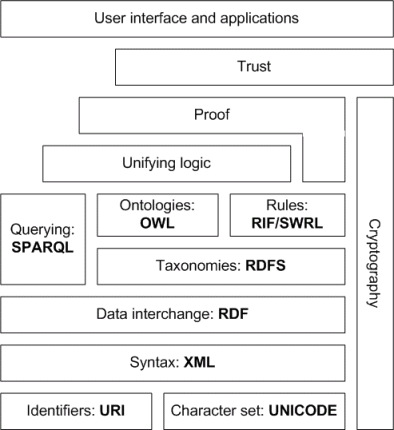
\includegraphics[width=0.5\linewidth]{./Figures/Semantic-web-stack.png}
\end{center}
\caption{Semantic Web stack}
\end{figure}

\begin{itemize}
 \item Resource Description Framework (RDF): a framework for creating statements in the form of triples composed by
subject, predicate and object. It uses URIs to name the predicates as well as the entities, which may be the subject or
object in a triple. RDF can be encoded in a variety of formats, such as RDF/XML, N3, Turtle and N-Triples.
 \item RDF Schema (RDFS): a RDF vocabulary description language which provides basic elements for the description of
ontologies (or RDF vocabularies) intended to structure RDF resources known as constructs (RDFS classes, associated
properties, and utility properties).
 \item Web Ontology Language (OWL): a semantic markup language for publishing and sharing ontologies on the web. It is a
vocabulary extension of RDF that allows an ontology to be described with a set of axioms which places constraints on
classes and the types of relationships permitted between them.
 \item SPARQL: an RDF query language for databases which can be used to express queries across diverse data sources. It
consists of triple patterns, conjunctions, disjunctions and optional patterns. 
 \item Rule Interchange Format (RIF): defines a standard for exchanging rules among rule systems. It focuses on
exchange rather than defining a single one-fits-all rule language, different databases might have different
characteristics with different necessities.
  \item Semantic Web Rule Language (SWRL): a proposal for rule language combining sublanguages of OWL with the
Unary/Binary Datolog Rule Markup Language (RuleML).
\end{itemize}

\section{Linked Open Data Applications}

The Semantic Web does not need only access to reachable and manageable data in a standard format, but also
relationships among data from different sources. Therewith, it is possible to create a huge collection of interrelated
datasets in the Web, also referred as Linked Data.

Linked Data is a fundamental part of the Semantic Web essence, facilitating a large scale integration and reasoning
on data on the Web. A typical example of Linked dataset is DBpedia
{\footnote{\url{http://www.dbpedia.org/}}}. It basically extracts information from Wikipedia and
make it available in RDF incorporating links to other datasets on the web, such as 
Geonames\footnote{\url{http://www.geonames.org/}},
YAGO\footnote{\url{http://www.mpi-inf.mpg.de/yago-naga/yago/}}, 
LinkedMDB\footnote{\url{http://www.linkedmdb.org/}} and 
USCensus\footnote{\url{http://www.linkedmdb.org/}}. 
With such linkage, it allows
applications to exploit the extra information these datasets can provide, integrating facts from various different
sources. Figure \ref{fig:lod} shows the Linked Open Data cloud
diagram, 

\begin{figure}
\label{fig:lod}
\begin{center}
  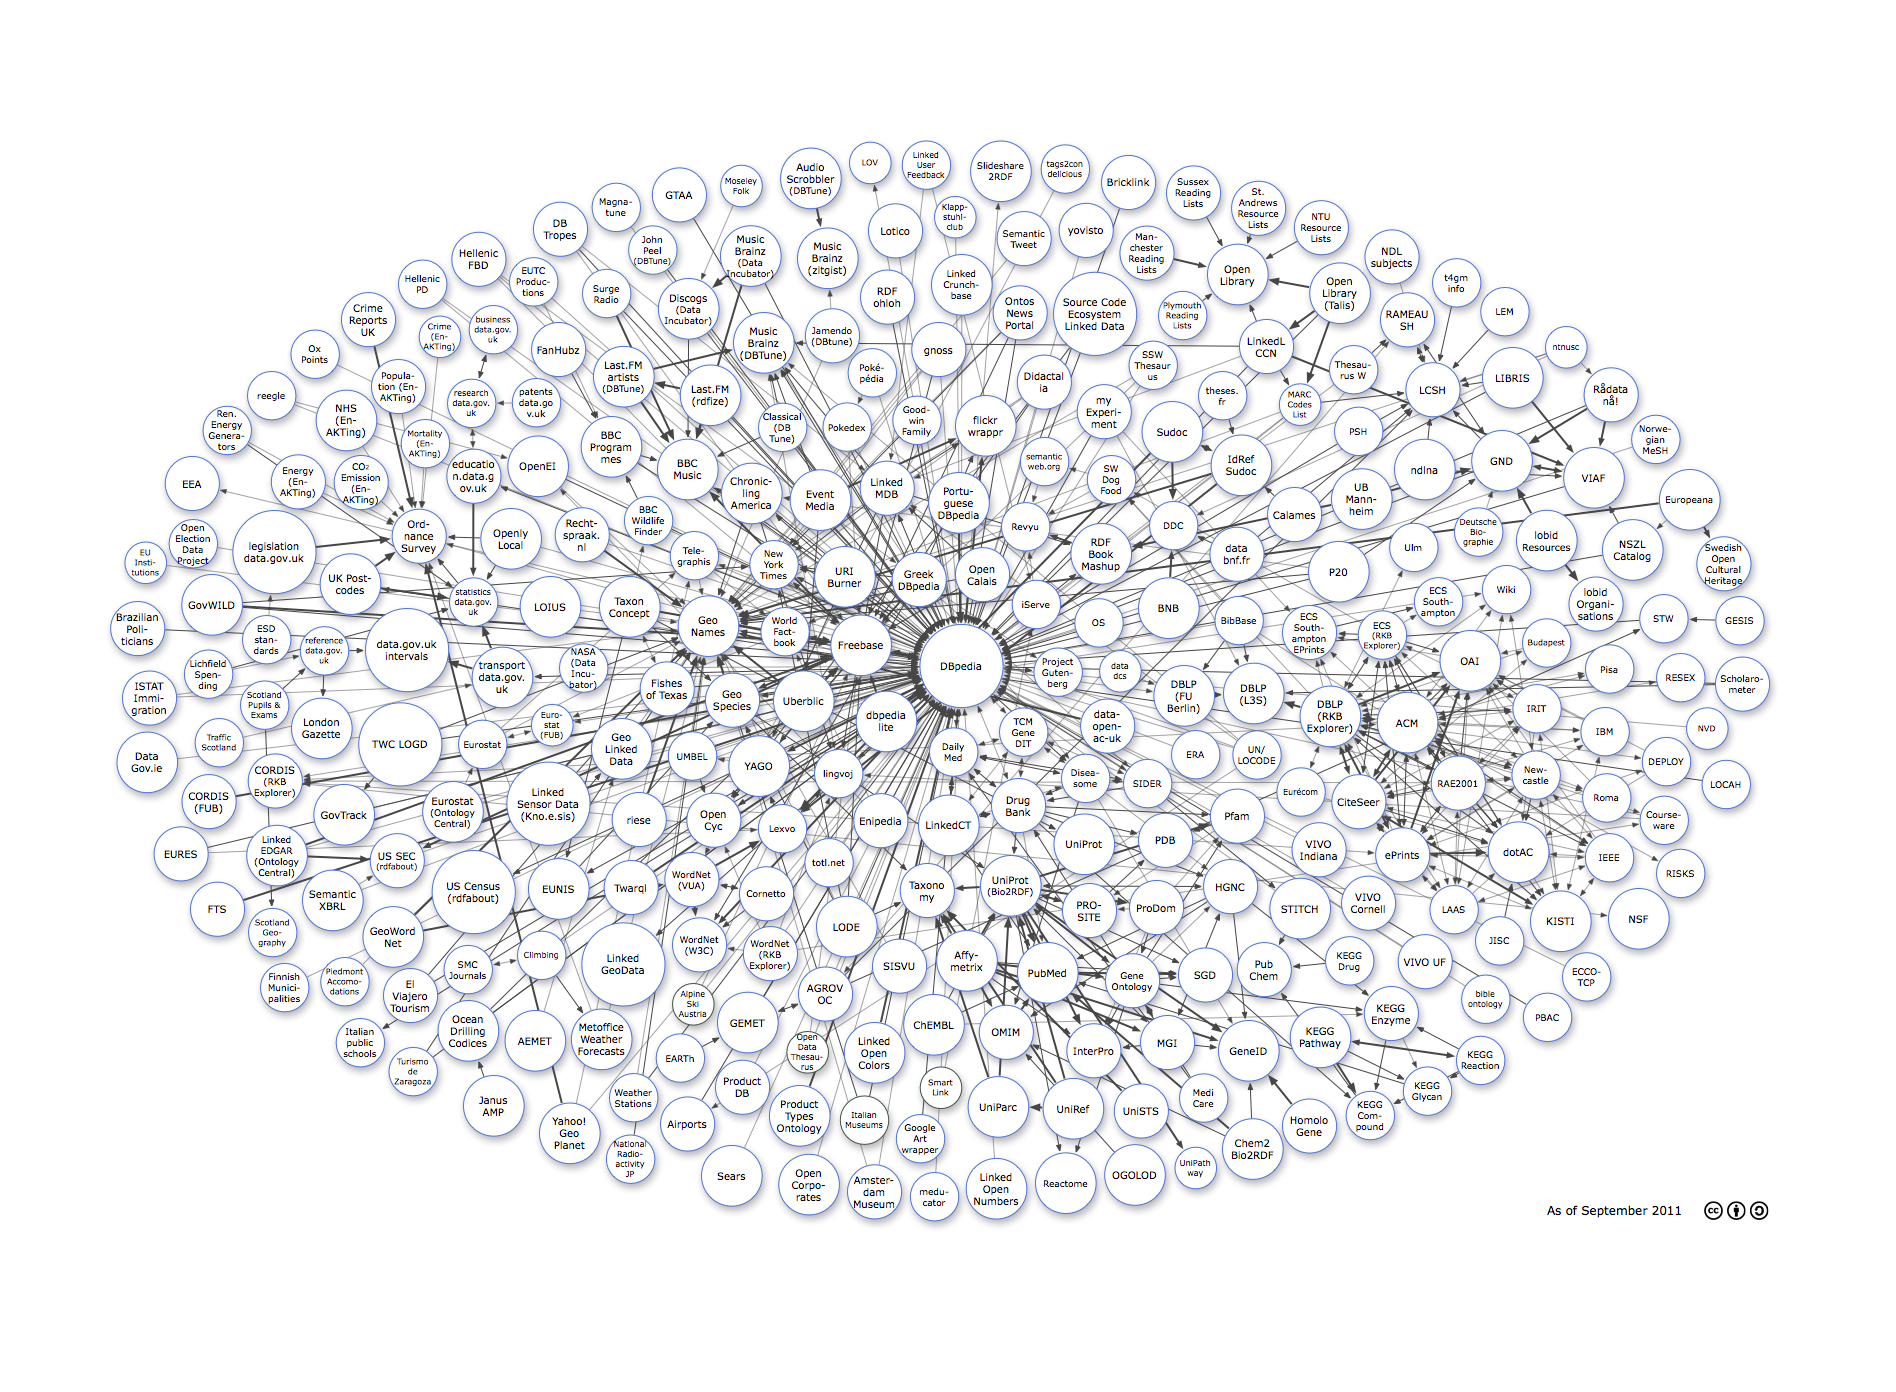
\includegraphics[width=1\linewidth]{./Figures/lod-datasets_2011-09-19.png}
\end{center}
\caption{Linking Open Data cloud diagram, by Richard Cyganiak and Anja Jentzsch. \url{http://lod-cloud.net}}
\end{figure}